%\documentclass[a4paper]{jarticle} 
\documentclass[dvipdfmx,a4paper]{jsarticle}
\usepackage{tikz}
\usepackage{amsmath}
\usepackage{amssymb}
\usepackage{comment}
\topmargin = 0mm
\oddsidemargin = 5mm
\textwidth = 152mm
\textheight = 240mm


% サブセクションを 問1,問2 にする設定
\renewcommand{\thesection}{[\arabic{section}]}

% サブサブセクションを (1),(2)にする設定
\renewcommand{\thesubsection}{(\arabic{subsection})}
% (i),(ii)なら \arabic を \roman に変える。    (a),(b)なら \alph

\renewcommand{\thesubsubsection}{(\roman{subsubsection})}

% 大問2の3番目の計算式のラベルを (2.3) にする設定
% 計算式の参照には \eqref{eq:hoge} を使う
\makeatletter
  \renewcommand{\theequation}{\arabic{subsection}.\arabic{equation}}
  \@addtoreset{equation}{subsection}
\makeatother

% --------------------------------------------------------------------
\begin{document}

% タイトル
\begin{center}
\textbf{\huge{数学2D演習 第3回}}
\end{center}

%名前
\begin{flushright}
工学部電気電子工学科3年 03200489 末吉七海\\
\end{flushright}

% --------------------------------------------------------------------
% 問1
\section{Cauchy-Riemannの関係式}

%(1)
\subsection{}

\subsubsection{$\bar{z}$}
\begin{align*}
\bar{z} &= x - iy\\
\therefore \quad u &= x \qquad v = -y\\
\therefore \quad \frac{\partial u}{\partial x} &= 1 \qquad \frac{\partial v}{\partial y} = -1
\end{align*}
以上より、$\mbox{\large $\frac{\partial u}{\partial x} \neq \frac{\partial v}{\partial y}$}$なので$\bar{z}$は正則でないと言える。

\subsubsection{$\exp{(\mbox{\large $\frac{1}{z}$})}$}
\begin{align*}
\frac{1}{z} &= \frac{1}{x + iy} = \frac{x-iy}{x^2 + y^2}\\
\therefore \quad \exp{\Bigl(\frac{1}{z}\Bigr)} &=  \exp{\Bigl(\frac{x}{x^2 + y^2} - i \frac{y}{x^2 + y^2}\Bigr)}\\
&= \exp{\Bigl(\frac{x}{x^2 + y^2}\Bigr)} \cos{\frac{y}{x^2 + y^2}} - i \exp{\Bigl(\frac{x}{x^2 + y^2}\Bigr)} \sin{\frac{y}{x^2 + y^2}}\\
\therefore \quad u &= \exp{\Bigl(\frac{x}{x^2 + y^2}\Bigr)} \cos{\frac{y}{x^2 + y^2}} \qquad v = -\exp{\Bigl(\frac{x}{x^2 + y^2}\Bigr)} \sin{\frac{y}{x^2 + y^2}}\\
\therefore \quad \frac{\partial u}{\partial x} &= \frac{-x^2+y^2}{(x^2+y^2)^2}\exp{\Bigl(\frac{x}{x^2 + y^2}\Bigr)} \cos{\frac{y}{x^2 + y^2}} + \frac{-2xy}{(x^2+y^2)^2}\exp{\Bigl(\frac{x}{x^2 + y^2}\Bigr)} \sin{\frac{y}{x^2 + y^2}}\\
\frac{\partial v}{\partial y} &= \frac{-x^2+y^2}{(x^2+y^2)^2}\exp{\Bigl(\frac{x}{x^2 + y^2}\Bigr)} \cos{\frac{y}{x^2 + y^2}} + \frac{-2xy}{(x^2+y^2)^2}\exp{\Bigl(\frac{x}{x^2 + y^2}\Bigr)} \sin{\frac{y}{x^2 + y^2}}
\end{align*}
以上より、$\mbox{\large $\frac{\partial u}{\partial x} = \frac{\partial v}{\partial y}$}$なので$\exp{(\mbox{\large $\frac{1}{z}$})}$は正則であると言える。ただし$z=0$を除く。

\subsubsection{$\cos{z}$}
\begin{align*}
\cos{z} &= \frac{e^iz + e^{-iz}}{2}\\
&= \frac{\exp{(ix - y)} + \exp{(-ix + y)}}{2}\\
&= \frac{e^{-y}(\cos{x} + i\sin{x}) + e^{y}(\cos{x} -i \sin{x})}{2}\\
&= \frac{e^{-y}\cos{x} + e^{y}\cos{x}}{2} + i\frac{e^{-y}\sin{x} - e^{y}\sin{x}}{2}\\
\therefore \quad u &= \frac{e^{-y}\cos{x} + e^{y}\cos{x}}{2} \qquad v = \frac{e^{-y}\sin{x} - e^{y}\sin{x}}{2}\\
\therefore \quad \frac{\partial u}{\partial x} &= \frac{-e^{-y}\sin{x} - e^{y}\sin{x}}{2}  \qquad \frac{\partial v}{\partial y} = \frac{-e^{-y}\sin{x} - e^{y}\sin{x}}{2}
\end{align*}
以上より、$\mbox{\large $\frac{\partial u}{\partial x} = \frac{\partial v}{\partial y}$}$なので$\cos{z}$は正則であると言える。

\subsubsection{$\mbox{\large $z^{\frac{1}{2}}$}$}
\begin{align*}
\mbox{\large $z^{\frac{1}{2}}$} &= \mbox{\large $r^{\frac{1}{2}}$}\exp{\Bigl(\frac{i\theta}{2}\Bigr)}\\
&= \mbox{\large $r^{\frac{1}{2}}$}\cos \Bigl(\frac{\theta}{2}\Bigr) + i \mbox{\large $r^{\frac{1}{2}}$}\sin \Bigl(\frac{\theta}{2}\Bigr)\\
\therefore \quad u &= \mbox{\large $r^{\frac{1}{2}}$}\cos \Bigl(\frac{\theta}{2}\Bigr) \qquad v = \mbox{\large $r^{\frac{1}{2}}$}\sin \Bigl(\frac{\theta}{2}\Bigr)\\
\therefore \quad \frac{\partial u}{\partial r} &= \frac{1}{2}\mbox{\large $r^{-\frac{1}{2}}$}\cos{(\frac{\theta}{2})} \qquad \frac{1}{r}\frac{\partial v}{\partial \theta} = \frac{1}{2} \mbox{\large $r^{-\frac{1}{2}}$}\cos \Bigl(\frac{\theta}{2}\Bigr)
\end{align*}
以上より、$\mbox{\large $\frac{\partial u}{\partial r} = \frac{1}{r}\frac{\partial v}{\partial \theta}$}$なので$\mbox{\large $z^{\frac{1}{2}}$}$は正則であると言える。ただし、$r=0$を除く。\\

%(2)
\subsection{}
$f(z) = u+iv $とおくと、$u=const.$\\
f(z)は正則より、 CR方程式から、
$$
\partial_y v = \partial_x u = 0
$$
ゆえに、$v=const.$\\
実部も虚部も定数より、f(z)は定数であるとことがわかる。\\

%(3)
\subsection{}
$f(z) = u+iv $とおくと、偏角が定数すなわち、$\mbox{\large $\frac{v}{u}$} = const.$\\
\begin{align*}
\therefore \quad \partial_x \frac{v}{u} &= \frac{u\partial_x v - v\partial_x u}{u^2} = 0\\
\partial_y \frac{v}{u} &= \frac{u\partial_y v - v\partial_y u}{u^2} = 0
\end{align*}
さらに、f(x)は正則より、CR方程式が成り立つので、
\begin{align*}
\partial_x u = \partial_y v \\
\partial_x v = -\partial_y u
\end{align*}
以上4つの式を連立すると、
\begin{align*}
\partial_x u = \partial_y v = \partial_x v = \partial_y u = 0\\
\therefore \quad u = const. \qquad v = const.
\end{align*}
よって、実部も虚部も定数より、f(z)は定数であるとことがわかる。\\

\newpage

%[2]
\section{複素積分のwarming up}
\begin{flushleft}
(a)
\end{flushleft}
$z = t(1+i)$とおくと、積分範囲は$0 \leq t \leq 1、\mathrm{dz} = (1+i)\mathrm{dt}$より、
\begin{align*}
\int_{\gamma}\mathrm{dz} \, x = \int^{1}_{0} (1+i) \mathrm{dt}\,  t = \frac{1+i}{2}
\end{align*}
\\

\begin{flushleft}
(b)
\end{flushleft}
$z = re^{i\theta}$とおくと、積分範囲は$0 \leq t \leq 2\pi、\mathrm{dz} = ire^{i\theta}\mathrm{d}\theta$より、
\begin{align*}
\int_{\gamma}\mathrm{dz}\,  x &= \int^{2\pi}_{0} ire^{i\theta}\mathrm{d\theta}\,  r \cos{\theta}\\
&= ir^2\int^{2\pi}_{0} \cos^2{\theta} \mathrm{d\theta}\\
&= i\pi r^2
\end{align*}
\\

\begin{flushleft}
(c)
\end{flushleft}
$z = re^{i\theta}$とおくと、積分範囲は$0 \leq t \leq 2\pi、\mathrm{d\bar{z}} = -ire^{-i\theta}\mathrm{d}\theta$より、
\begin{align*}
\int_{\gamma}\mathrm{dz} \, z &= \int^{2\pi}_{0} -ire^{-i\theta} \mathrm{d\theta} \, re^{i\theta}\\
&= -ir^2\int^{2\pi}_{0} \mathrm{d\theta}\\
&= -2i\pi r^2
\end{align*}
\\

\begin{flushleft}
(d)
\end{flushleft}
$z = re^{i\theta}$とおくと、積分範囲は$0 \leq t \leq 2\pi、\mathrm{d\bar{z}} = -ire^{-i\theta}\mathrm{d}\theta$より、
\begin{align*}
\int_{\gamma}\mathrm{dz}\,  z &= \int^{2\pi}_{0} -ire^{-i\theta} \mathrm{d\theta} \, \frac{1}{r}e^{-i\theta}\\
&= -i\int^{2\pi}_{0} e^{-2i\theta} \mathrm{d\theta}\\
&= 0
\end{align*}
\\


%[3]
\section{Cauchyの積分定理}

%(1)
\subsection{}
$z = 2e^{i\theta}$とおくと、積分範囲は$0 \leq t \leq 2\pi、\mathrm{dz} = 2ie^{i\theta}\mathrm{d}\theta$より、
\begin{align*}
\int_{C_1}z^2\mathrm{dz} = \int^{2\pi}_{0} 4e^{2i\theta} 2ie^{i\theta}\mathrm{d}\theta = \int^{2\pi}_{0} 8ie^{3i\theta}\mathrm{d}\theta = 0\\
\end{align*}

%(2)
\subsection{}
$z = 2e^{i\theta}$とおくと、積分範囲は$0 \leq t \leq 2\pi、|\mathrm{dz}| = 2\mathrm{d}\theta$より、
\begin{align*}
\int_{C_1}z^2|\mathrm{dz}| = \int^{2\pi}_{0} 4e^{2i\theta}2\mathrm{d}\theta = \int^{2\pi}_{0} 8e^{2i\theta}\mathrm{d}\theta = 0\\
\end{align*}

%(3)
\subsection{}
$z = 2e^{i\theta}$とおくと、積分範囲は$0 \leq t \leq 2\pi、|\mathrm{dz}| = 2\mathrm{d}\theta$より、
\begin{align*}
\int_{C_1}z^2|\mathrm{dz}| = \int^{2\pi}_{0} 4 \times 2\mathrm{d}\theta = \int^{2\pi}_{0} 8\mathrm{d}\theta = 16\pi\\
\end{align*}

%(4)
\subsection{}
$z = 2e^{i\theta}$とおくと、積分範囲は$0 \leq t \leq \mbox{\large$\frac{\pi}{2}$}、\mathrm{dz} = 2ie^{i\theta}\mathrm{d}\theta$より、
\begin{align*}
\int_{C_2}\frac{1}{z}\mathrm{dz} = \int^{\frac{\pi}{2}}_{0}\frac{1}{2}e^{-i\theta} 2ie^{i\theta} \mathrm{d}\theta = \int^{\frac{\pi}{2}}_{0} i\mathrm{d}\theta = \frac{i}{2}\\
\end{align*}

%(5)
\subsection{}
$z = 2e^{i\theta}$とおくと、積分範囲は$\mbox{\large$\frac{\pi}{2}$} \leq t \leq 2\pi、\mathrm{dz} = 2ie^{i\theta}\mathrm{d}\theta$より、
\begin{align*}
\int_{C_3}\frac{1}{z}\mathrm{dz} = \int^{2\pi}_{\frac{\pi}{2}}\frac{1}{2}e^{-i\theta} 2ie^{i\theta} \mathrm{d}\theta = \int^{2\pi}_{\frac{\pi}{2}} i\mathrm{d}\theta = \frac{3\pi}{2}i\\
\end{align*}

%(6)
\subsection{}
$\mbox{\Large$\frac{\pi}{2}$}$の特異点は$z=0$であり、$C_3$の積分経路に沿った向きで左手に存在するので、
\begin{align*}
\int_{C_4}\frac{1}{z}\mathrm{dz} = \int_{C_3}\frac{1}{z}\mathrm{dz} = \frac{3\pi}{2}i\\
\end{align*}

%(7)
\subsection{}
\,0から1において、$z = t$とおくと、積分範囲は$0 \leq t \leq 1\pi、\mathrm{dz} = \mathrm{dt}$\\
 1から$1+i$において、$z = 1+ti$とおくと、積分範囲は$0 \leq t \leq 1\pi、\mathrm{dz} = i\mathrm{dt}$
\begin{align*}
\int_{C_5}|z|^2\mathrm{dz} &= \int_{0}^{1}t^2\mathrm{dt} + \int_{0}^{1}|1+ti|^2i\mathrm{dt}
= \int_{0}^{1}t^2\mathrm{dt} + \int_{0}^{1}(1+t^2)i\mathrm{dt} 
= \frac{1}{3} + i\frac{4}{3}\\
\end{align*}

%(8)
\subsection{}
\,0からiにおいて、$z = ti$とおくと、積分範囲は$0 \leq t \leq 1\pi、\mathrm{dz} = i\mathrm{dt}$\\
 iから$1+i$において、$z = t+i$とおくと、積分範囲は$0 \leq t \leq 1\pi、\mathrm{dz} = \mathrm{dt}$
\begin{align*}
\int_{C_6}|z|^2\mathrm{dz} &= \int_{0}^{1}|ti|^2i\mathrm{dt} + \int_{0}^{1}|t+i|^2\mathrm{dt}
= \int_{0}^{1}t^2i\mathrm{dt} + \int_{0}^{1}(1+t^2)\mathrm{dt} 
= \frac{4}{3} + i\frac{1}{3}\\\\
\end{align*}


%[4]
\section{複素平面間の写像}

%(1)
\subsection{}
$z = x+iy、w = u+iv$とおくと、
\begin{align*}
w = z^2 &= (x+iy)^2 = (x^2-y^2) + i2xy\\
\therefore \quad u &= x^2-y^2 \qquad v = 2xy\\
\therefore \quad u &= - \bigl(\frac{v}{2x}\bigr)^2 + x^2 \qquad u =  \bigl(\frac{v}{2y}\bigr)^2 - y^2
\end{align*}
よってw座標に図示すると、下の図のような放物線群となる。ただし、実軸の負の部分は除く。

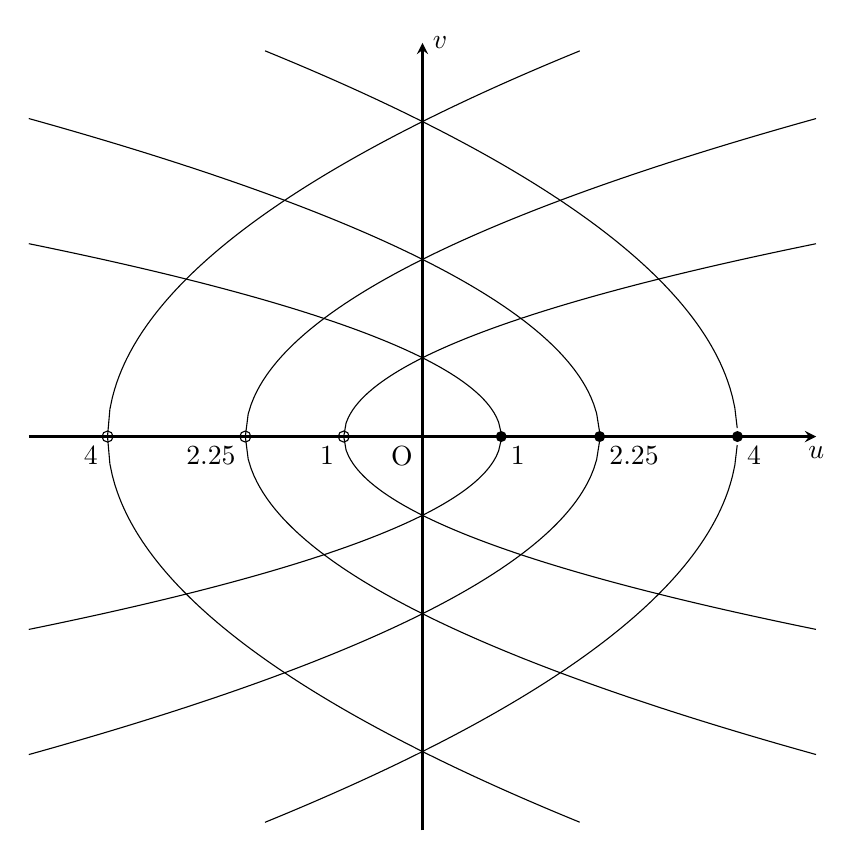
\begin{tikzpicture}
 \coordinate[label=below left:O] (O) at (0,0); %原点O
 \coordinate (XS) at (-5,0); %x軸最小
 \coordinate (XL) at (5,0); %x軸最大
 \coordinate (YS) at (0,-5); %y軸最小
 \coordinate (YL) at (0,5); %y軸最大
 \draw[thick,->,>=stealth] (XS)--(XL) node[below] {$u$}; %x軸
 \draw[thick,->,>=stealth] (YS)--(YL) node[right] {$v$}; %y軸
 
 \draw [samples = 200, domain=-5:1] plot(\x, {sqrt(1-\x)});
 \draw [samples = 200, domain=-5:1] plot(\x, {-sqrt(1-\x)});
 \draw [samples = 200, domain=-1:5] plot(\x, {sqrt(1+\x)});
 \draw [samples = 200, domain=-1:5] plot(\x, {-sqrt(1+\x)});
 \draw [samples = 200, domain=-2:4] plot(\x, {2*sqrt(4-\x)});
 \draw [samples = 200, domain=-2:4] plot(\x, {-2*sqrt(4-\x)});
 \draw [samples = 200, domain=-4:2] plot(\x, {2*sqrt(4+\x)});
 \draw [samples = 200, domain=-4:2] plot(\x, {-2*sqrt(4+\x)});
 \draw [samples = 200, domain=-5:2.25] plot(\x, {1.5*sqrt(2.25-\x)});
 \draw [samples = 200, domain=-5:2.25] plot(\x, {-1.5*sqrt(2.25-\x)});
 \draw [samples = 200, domain=-2.25:5] plot(\x, {1.5*sqrt(2.25+\x)});
 \draw [samples = 200, domain=-2.25:5] plot(\x, {-1.5*sqrt(2.25+\x)});
 \coordinate[label=below right:1] (A) at (1,0);
 \coordinate[label=below right:2.25] (B) at (2.25,0);
 \coordinate[label=below right:4] (C) at (4,0);
 \coordinate[label=below left:1] (D) at (-1,0);
 \coordinate[label=below left:2.25] (E) at (-2.25,0);
 \coordinate[label=below left:4] (F) at (-4,0);
 \fill (A) circle(0.07);
 \fill (B) circle(0.07);
 \fill (C) circle(0.07);
 \draw (D) circle [radius = 0.07];
 \draw (E) circle [radius = 0.07];
 \draw (F) circle [radius = 0.07];
\end{tikzpicture}
\\

%(2)
\subsection{}
\subsubsection{}
zからwへ一次分数変換を行うと、$a,b,c,d\in \mathbb{C}$として、
\begin{align*}
w &= \frac{az+b}{cz+d} \\
&= \frac{\frac{a}{c}z + \frac{b}{c}}{z + \frac{d}{c}}\\
&= \frac{a}{c} + \frac{\frac{b}{c}-\frac{ad}{c}}{z + \frac{d}{c}}\\
&= \frac{a}{c} + \frac{\frac{bc-ad}{c^2}}{z + \frac{d}{c}}
\end{align*}
よって、\\
1. $\mbox{\large $\frac{d}{c}$}$平行移動\\
2. 原点対称移動\\
3. $\mbox{\Large $\bigl|\frac{\frac{bc-ad}{c^2}}{c^2}\bigr|$}$拡大\\
4. 原点中心にarg$\biggl[\mbox{\Large $\frac{\frac{bc-ad}{c^2}}{c^2}$}\biggr]$回転\\
5. $\mbox{\large $\frac{a}{c}$}$平行移動\\
以上の変換で、zからwへ一次分数変換を行うことが可能である。\\
ゆえに、円から円に変換することが可能であると言える。\\

\subsubsection{}
点$\alpha$を原点とおき、円$C_1, C_2$の半径をそれぞれ$a_1, a_2$とおくと、\\$C_1$上の点は$a_1 = |z+a_1|$、$C_2$上の点は$a_2 = |z+a_2|$と表せる。\\
ここで、wへの一次分数変換$\mbox{\large $\frac{1}{z-\alpha}$}$を考えると$C_1,C_2$はそれぞれ、\\
w上の直線$L_1:u = -\mbox{\large $\frac{1}{a_1}$}, L_2:u = -\mbox{\large $\frac{1}{a_2}$}, $へと変換される。\\

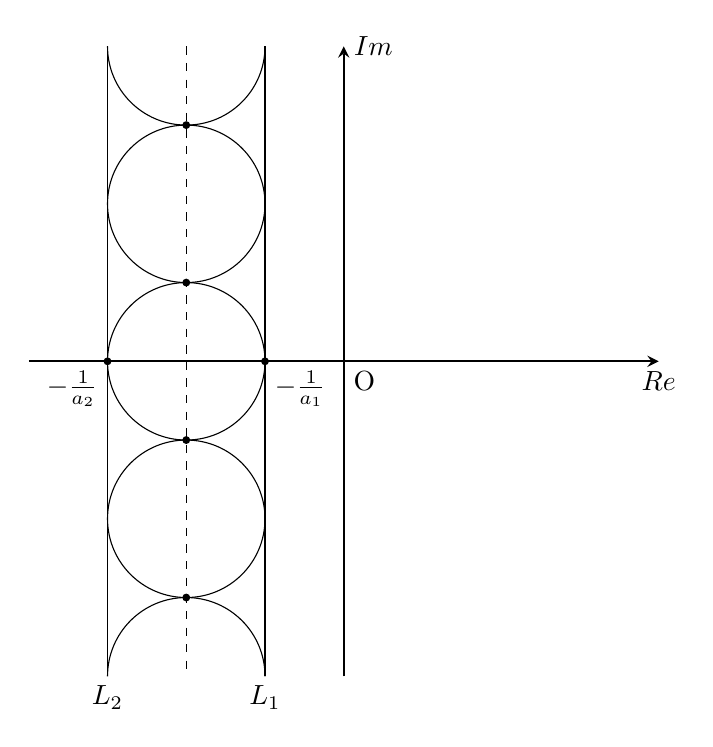
\begin{tikzpicture}
 \coordinate[label=below right:O] (O) at (0,0); %原点O
 \coordinate (XS) at (-4,0); %x軸最小
 \coordinate (XL) at (4,0); %x軸最大
 \coordinate (YS) at (0,-4); %y軸最小
 \coordinate (YL) at (0,4); %y軸最大
 \draw[thick,->,>=stealth] (XS)--(XL) node[below] {$Re$}; %x軸
 \draw[thick,->,>=stealth] (YS)--(YL) node[right] {$Im$}; %y軸
 
 \draw (-2,0) circle [radius = 1];
 \draw (-2,2) circle [radius = 1];
 \draw (-2,-2) circle [radius = 1];
 \draw (-3,4) arc (180:360:1);
 \draw (-1,-4) arc (0:180:1);
 \draw (-3,4)--(-3,-4);
 \draw (-1,4)--(-1,-4);
 \draw [dashed] (-2,4)--(-2,-4);
 \fill (-2,3) circle(0.05);
 \fill (-2,1) circle(0.05);
 \fill (-2,-1) circle(0.05);
 \fill (-2,-3) circle(0.05);
 \fill (-1,0) node[below right]{$-\frac{1}{a_1}$} circle(0.05);
 \fill (-3,0) node[below left]{$-\frac{1}{a_2}$} circle(0.05);
 \coordinate [label = below: $L_1$] (a) at (-1,-4);
 \coordinate [label = below: $L_2$] (a) at (-3,-4);
\end{tikzpicture}

$L_1, L_2$は上の図のようになり、$L_1, L_2$に接する円もこのように描ける。\\
これらの円の接点を結ぶと上の図の破線のような直線となり、その式は、
\begin{align*}
u &= \frac{1}{2}\bigl(-\frac{1}{a_1}-\frac{1}{a_2}\bigr) \\
\therefore \quad u &= -\frac{1}{2}\frac{1}{\frac{2a_1a_2}{a_1 + a_2}}
\end{align*}
z平面へ逆変換すると、
$$
\Bigl|z+\frac{2a_1a_2}{a_1 + a_2}\Bigr| = \frac{2a_1a_2}{a_1 + a_2}
$$
以上より、$C_1$と$C_2$に接する円同士の接点は、\\
$C_1$と$C_2$の中心の中点を中心として半径$\mbox{\large$\frac{2a_1a_2}{a_1 + a_2}$}$の円上にある。\\


%[5]
\section{複素平面間の写像}

%(1)
\subsection{}
$$
\mathrm{Log}(1+z) = z - \frac{1}{2}z^2 + \frac{1}{3}z^3 - \cdots + (-1)^n\frac{1}{n}z^n + \cdots
$$
収束するのは、
\begin{align*}
\lim_{n \to \infty}\biggl|\frac{(-1)^{n+1}\frac{1}{n+1}z^{n+1}}{(-1)^n\frac{1}{n}z^n}\biggr| &< 1\\
\therefore \quad \lim_{n \to \infty}\frac{n}{n+1}|z| &< 1\\
\therefore \quad |z| &< 1
\end{align*}
よって下の図のような円の内部になる。ただし境界を除く。\\

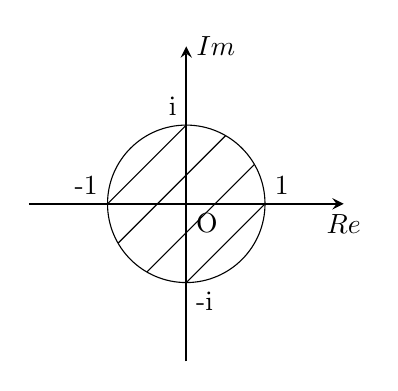
\begin{tikzpicture}
 \coordinate[label=below right:O] (O) at (0,0); %原点O
 \coordinate (XS) at (-2,0); %x軸最小
 \coordinate (XL) at (2,0); %x軸最大
 \coordinate (YS) at (0,-2); %y軸最小
 \coordinate (YL) at (0,2); %y軸最大
 \draw[thick,->,>=stealth] (XS)--(XL) node[below] {$Re$}; %x軸
 \draw[thick,->,>=stealth] (YS)--(YL) node[right] {$Im$}; %y軸
 
 \draw (0,0) circle [radius = 1];
 \draw (-1,0)--(0,1);
 \draw (0,-1)--(1,0);
 \draw ({-sqrt(3)/2}, -1/2)--(1/2,{sqrt(3)/2});
 \draw (-1/2, {-sqrt(3)/2})--({sqrt(3)/2},1/2);
 \coordinate [label=above left : i] (a) at (0,1);
 \coordinate [label=above left: -1] (a) at (-1,0);
 \coordinate [label=below right: -i] (a) at (0,-1);
 \coordinate [label=above right: 1] (a) at (1,0);
\end{tikzpicture}
\\

\subsection{}
境界は、$|w| = 1$であり、$w = \cos{\theta} + i\sin{\theta}(0 \leq \theta < 2\pi)$とおくと、
\begin{align*}
z &= \frac{2w}{1-w} = \frac{2\cos{\theta} + i2\sin{\theta}}{1 - \cos{\theta} - i\sin{\theta}}\\
&= \frac{(2\cos{\theta} + i\sin{\theta})(1 - \cos{\theta} + i\sin{\theta})}{2 - 2\cos{\theta}}\\ 
&= \frac{(2\cos{\theta} - 2) + i 2 \sin{\theta}}{2-2\cos{\theta}}\\
&= -1 + i\frac{\sin{\theta}}{1-\cos{\theta}}\\
&=-1 + i\frac{2\sin{\frac{\theta}{2}}\cos{\frac{\theta}{2}}}{2\sin^2{\frac{\theta}{2}}}\\
&=-1 + i\frac{\cos{\frac{\theta}{2}}}{\sin{\frac{\theta}{2}}}\\
&= -1 + i\cot{\frac{\theta}{2}}
\end{align*}
$0 \leq \theta < 2\pi$において、$-\infty \leq \cot{\mbox{\large$\frac{\pi}{2}$}} < \infty$であるから、z平面において境界は、直線$x = -1$である。\\
$|w| < 1$ は、$w = 0$を含むので、$z = \mbox{\large$\frac{0}{1-0}$} = 0$を含む。\\
よって、下の図のx = -1の右側であり、境界は含まない。\\

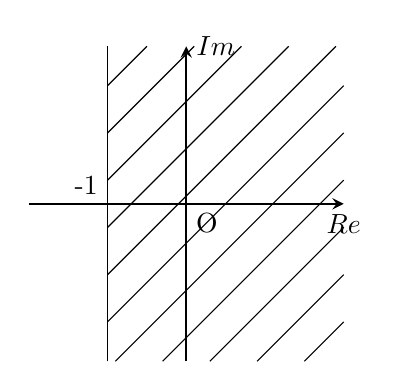
\begin{tikzpicture}
 \coordinate[label=below right:O] (O) at (0,0); %原点O
 \coordinate (XS) at (-2,0); %x軸最小
 \coordinate (XL) at (2,0); %x軸最大
 \coordinate (YS) at (0,-2); %y軸最小
 \coordinate (YL) at (0,2); %y軸最大
 \draw[thick,->,>=stealth] (XS)--(XL) node[below] {$Re$}; %x軸
 \draw[thick,->,>=stealth] (YS)--(YL) node[right] {$Im$}; %y軸
 
 \draw (-1,-2)--(-1,2);
 \draw (-1, 1.5)--(-0.5,2);
 \draw (-1, 0.9)--(0.1,2);
 \draw (-1, 0.3)--(0.7,2);
 \draw (-1, -0.3)--(1.3,2);
 \draw (-1, -0.9)--(1.9,2);
 \draw (-1, -1.5)--(2, 1.5);
 \draw (-0.9, -2)--(2, 0.9);
 \draw (-0.3, -2)--(2, 0.3);
 \draw (0.3, -2)--(2, -0.3);
 \draw (0.9, -2)--(2, -0.9);
 \draw (1.5, -2)--(2, -1.5);
 \coordinate [label=above left: -1] (a) at (-1,0);
\end{tikzpicture}
\\

%(3)
\subsection{}
\begin{align*}
\mathrm{Log}(1+z) &= \mathrm{Log}\bigl(1+\frac{2w}{1-w}\bigr) = \mathrm{Log}\bigl(\frac{1+w}{1-w}\bigr) = \mathrm{Log}(1+w) - \mathrm{Log}(1-w)\\
&= w - \frac{1}{2}w^2 + \frac{1}{3}w^3 + \cdots - (-w - \frac{1}{2}w^2 -\frac{1}{3}w^3 + \cdots)\\
&= 2\bigl(w + \frac{1}{3}w^3 + \cdots + \frac{1}{2n+1}w^{2n+1} + \cdots \bigr)
\end{align*}
収束する領域は、
\begin{align*}
\lim_{n \to \infty} \frac{\bigl|\frac{2}{2(n+1)+1}w^{2(n+1)+1}\bigr|}{\bigl|\frac{2}{2n+1}w^{2n+1}\bigr|} < 1\\
\therefore \quad |w|^2 < 1
\end{align*}
よって、原点を中心として、半径1の円の内部で収束する。\\

%(4)
\subsection{}
$z = \mbox{\large$\frac{2w}{1-w}$}$より、$w = \mbox{\large$\frac{z}{2+z}$}$を(3)の級数展開に代入すると、
\begin{align*}
\mathrm{Log}(1+z) &= 2\bigl(w + \frac{1}{3}w^3 + \cdots + \frac{1}{2n+1}w^{2n+1} + \cdots \bigr)\\
&= 2\Bigl(\bigl(\frac{z}{2+z}\bigr) + \frac{1}{3}\bigl(\frac{z}{2+z}\bigr)^3 + \cdots + \frac{1}{2n+1}\bigl(\frac{z}{2+z}\bigr)^{2n+1} + \cdots \Bigr)
\end{align*}
収束する領域は、
\begin{align*}
|w| = \bigl|\frac{z}{2+z}\bigr| < 1\\
\therefore \quad z > -1
\end{align*}
よって、zの実部が-1より大きいときに収束する。

\end{document}